\section{Plots}

\subsection{Histogram of Gini sample}

\begin{figure}[H]
  \centering
  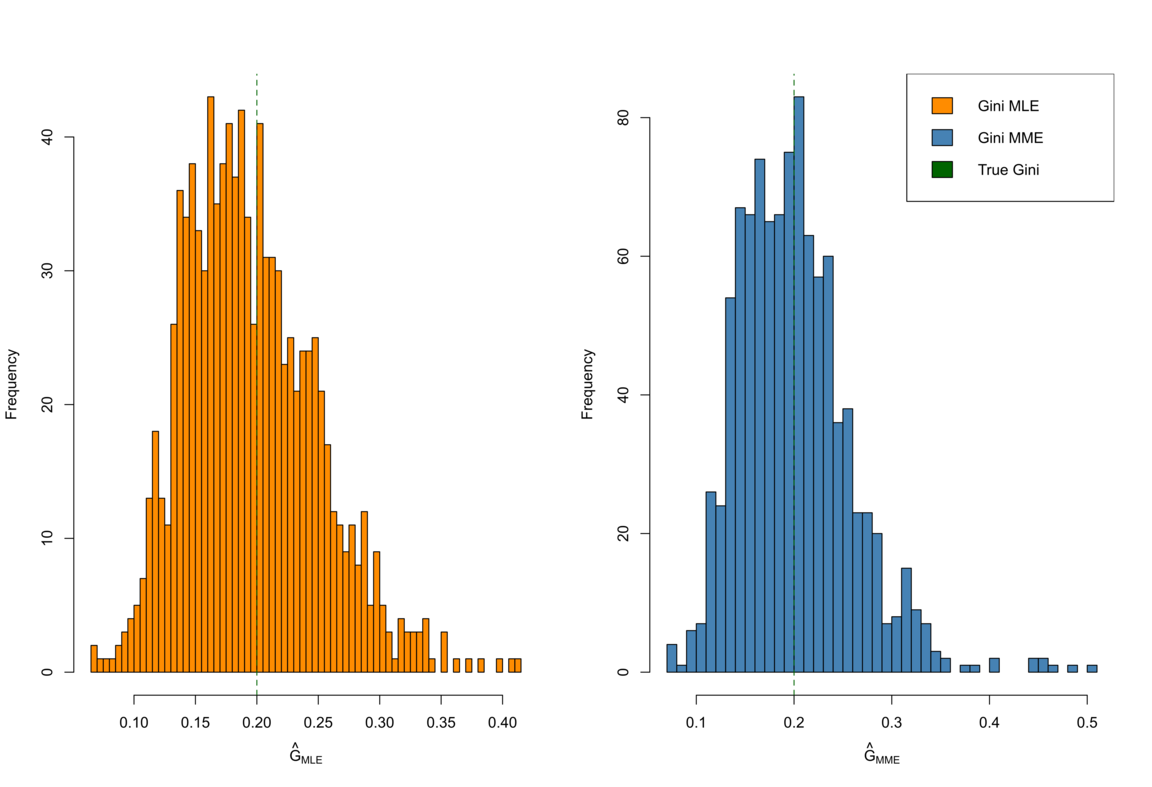
\includegraphics[width=\textwidth]{figures/png/gini_sample_histogram.png}
  \caption{histogram of $N = 1000$ simulations of Gini coefficients estimated by the maximum likelihood method (\textit{left}) and the moments method (\textit{right}) base on a sample of size $n = 20$. In green we have the exact value of the Gini coefficient}
  \label{fig:gini-sample-histogram-N=1000}
\end{figure}

\subsection{Boxplot of Gini sample}

\begin{figure}[H]
  \centering
  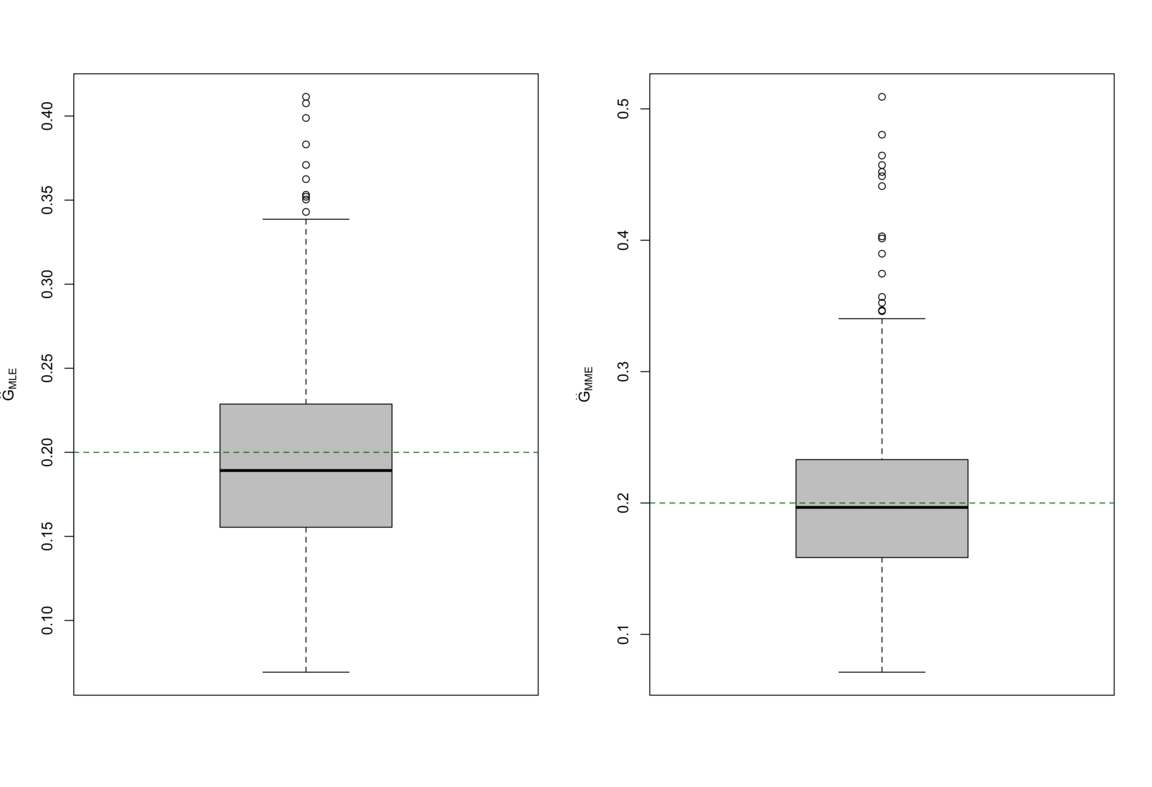
\includegraphics[width=\textwidth]{figures/png/gini_sample_boxplot.png}
  \caption{boxplot of $N = 1000$ simulations of Gini coefficients estimated by the maximum likelihood method (\textit{left}) and the moments method (\textit{right}) base on a sample of size $n = 20$. In green we have the exact value of the Gini coefficient}
  \label{fig:gini-sample-boxplot-N=1000}
\end{figure}

\subsection{Gini estimators: bias plot}

\begin{figure}[H]
  \centering
  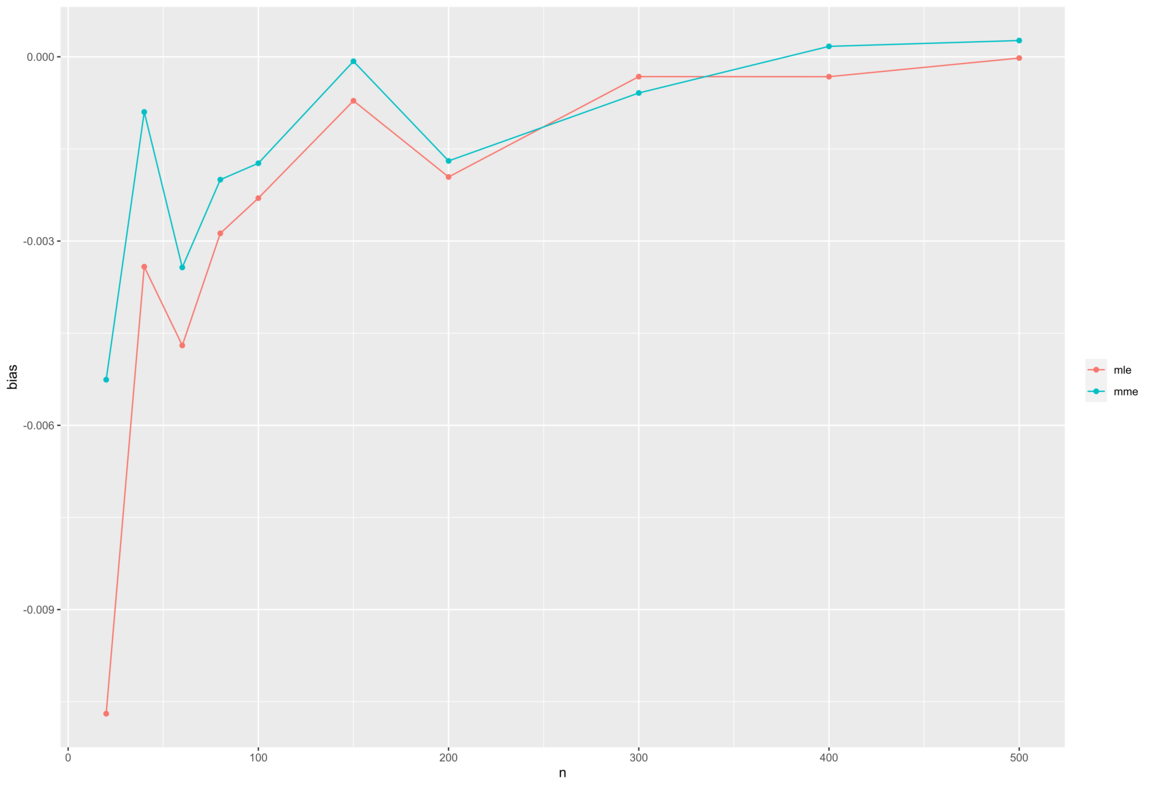
\includegraphics[width=\linewidth]{figures/png/gini_bias_plot.png}
  \caption{Plot of the bias of the Gini estimators (obtained by maximum likelihood in \textbf{red} and by method of moment in \textbf{turquoise}) as a function of the sample size $n$.}
  \label{fig:gini-estimators-bias-plot}
\end{figure}

\subsection{Gini estimators: variance plot}

\begin{figure}[H]
  \centering
  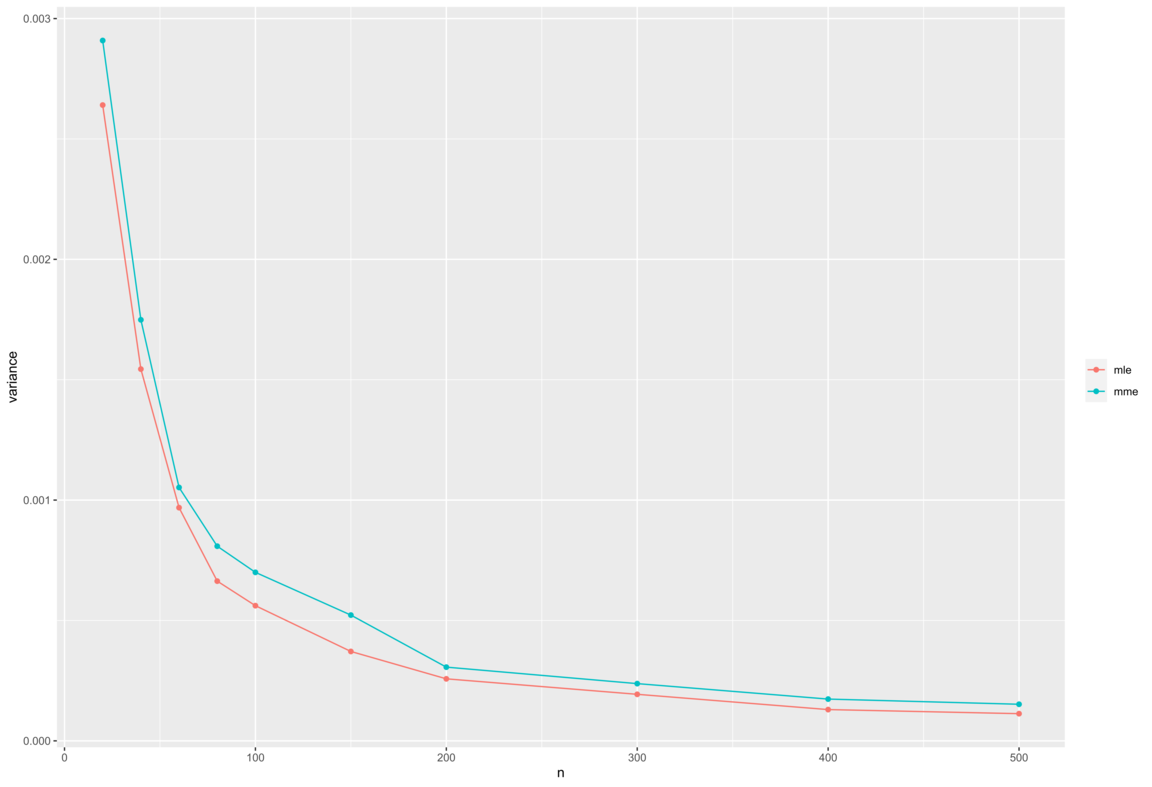
\includegraphics[width=\linewidth]{figures/png/gini_var_plot.png}
  \caption{Plot of the variance of the gini estimators (obtained by maximum likelihood in \textbf{red} and by method of moment in \textbf{turquoise}) as a function of the sample size $n$.}
  \label{fig:gini-estiamtors-variance-plot}
\end{figure}

\subsection{Gini estimators: mean squared error plot}

\begin{figure}[H]
  \centering
  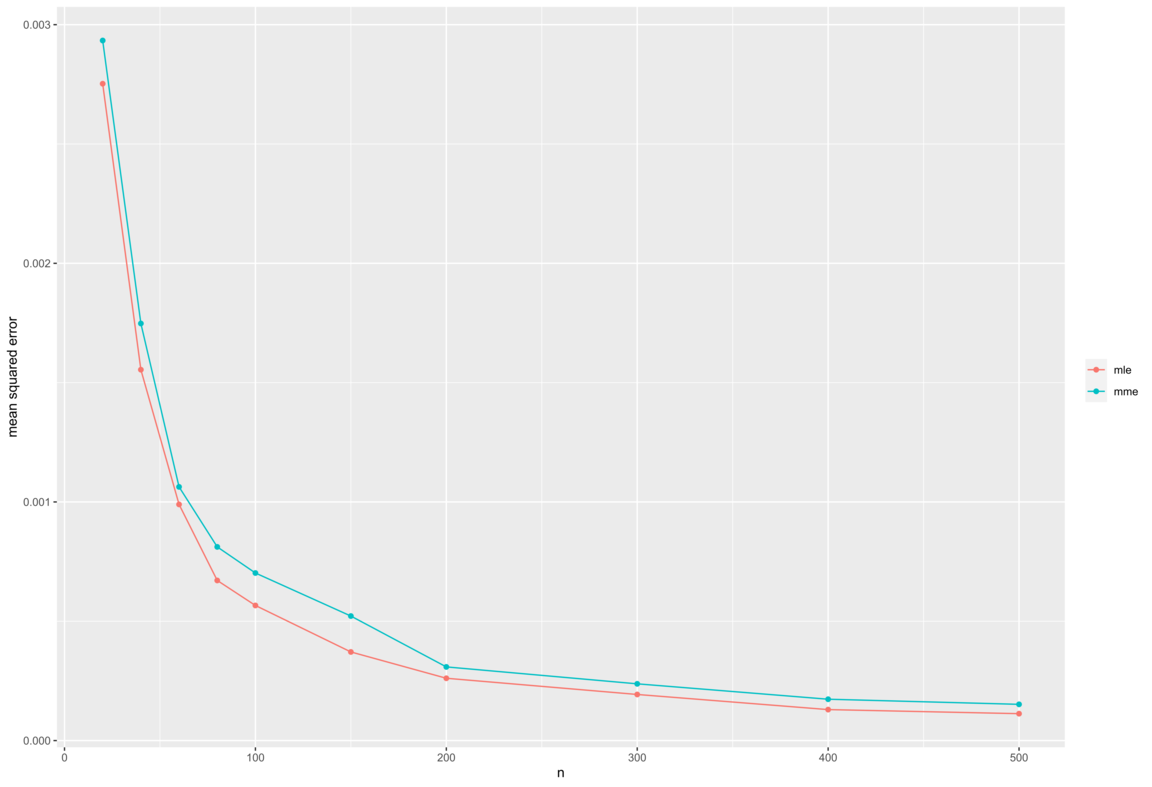
\includegraphics[width=\linewidth]{figures/png/gini_mse_plot.png}
  \caption{Plot of the mean squared error (MSE) of the gini estimators (obtained by maximum likelihood in \textbf{red} and by method of moment in \textbf{turquoise}) as a function of the sample size $n$.}
  \label{fig:gini-estimators-mse-plot}
\end{figure}

\subsection{Histograms of the formula (question (i))}

\begin{figure}[H]
  \centering
  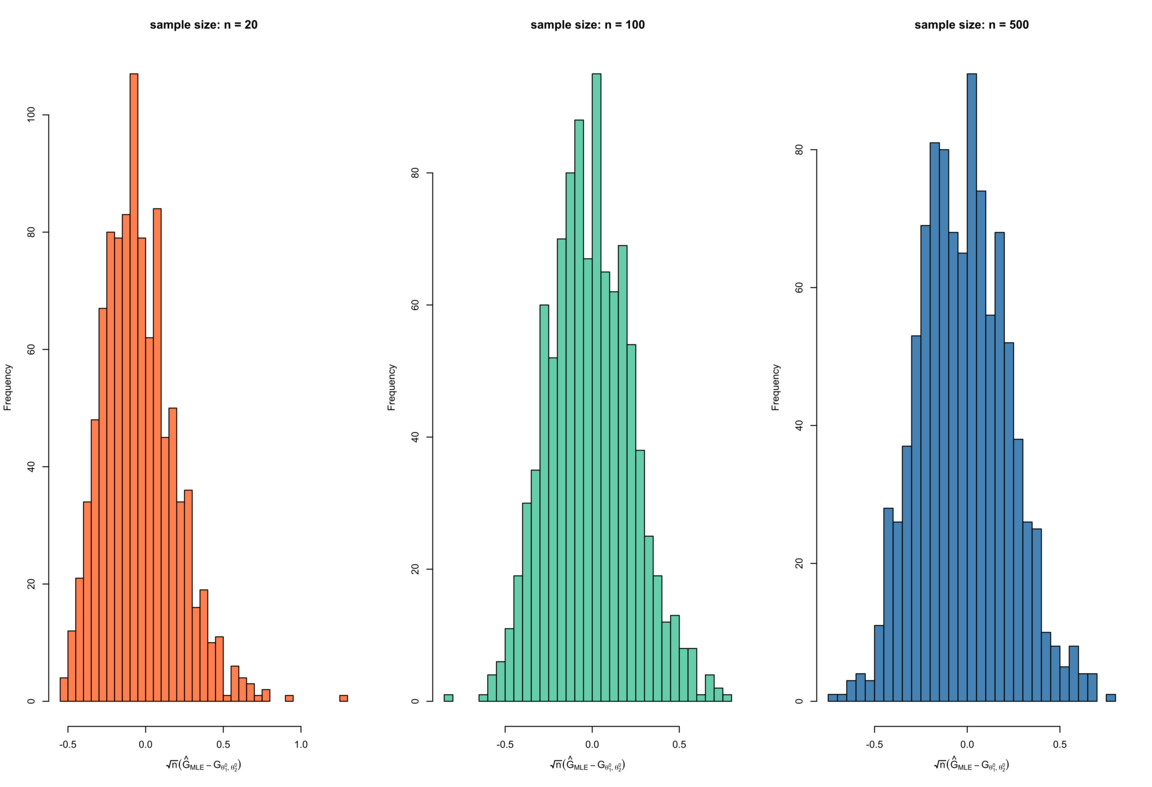
\includegraphics[width=\textwidth]{figures/png/special_formula_comparison.png}
  \caption{histogram for $\sqrt{n}(\hat{G}_{\text{MLE}} - G_{\theta_1^0, \theta_2^0})$, for sample size $n = 20$, $n = 100$ and $n = 500$}
  \label{fig:special-formula-sample-size-comparison}
\end{figure}

\subsection{Scatter plot of productivity vs electricity consumption}

\begin{figure}[H]
  \centering
  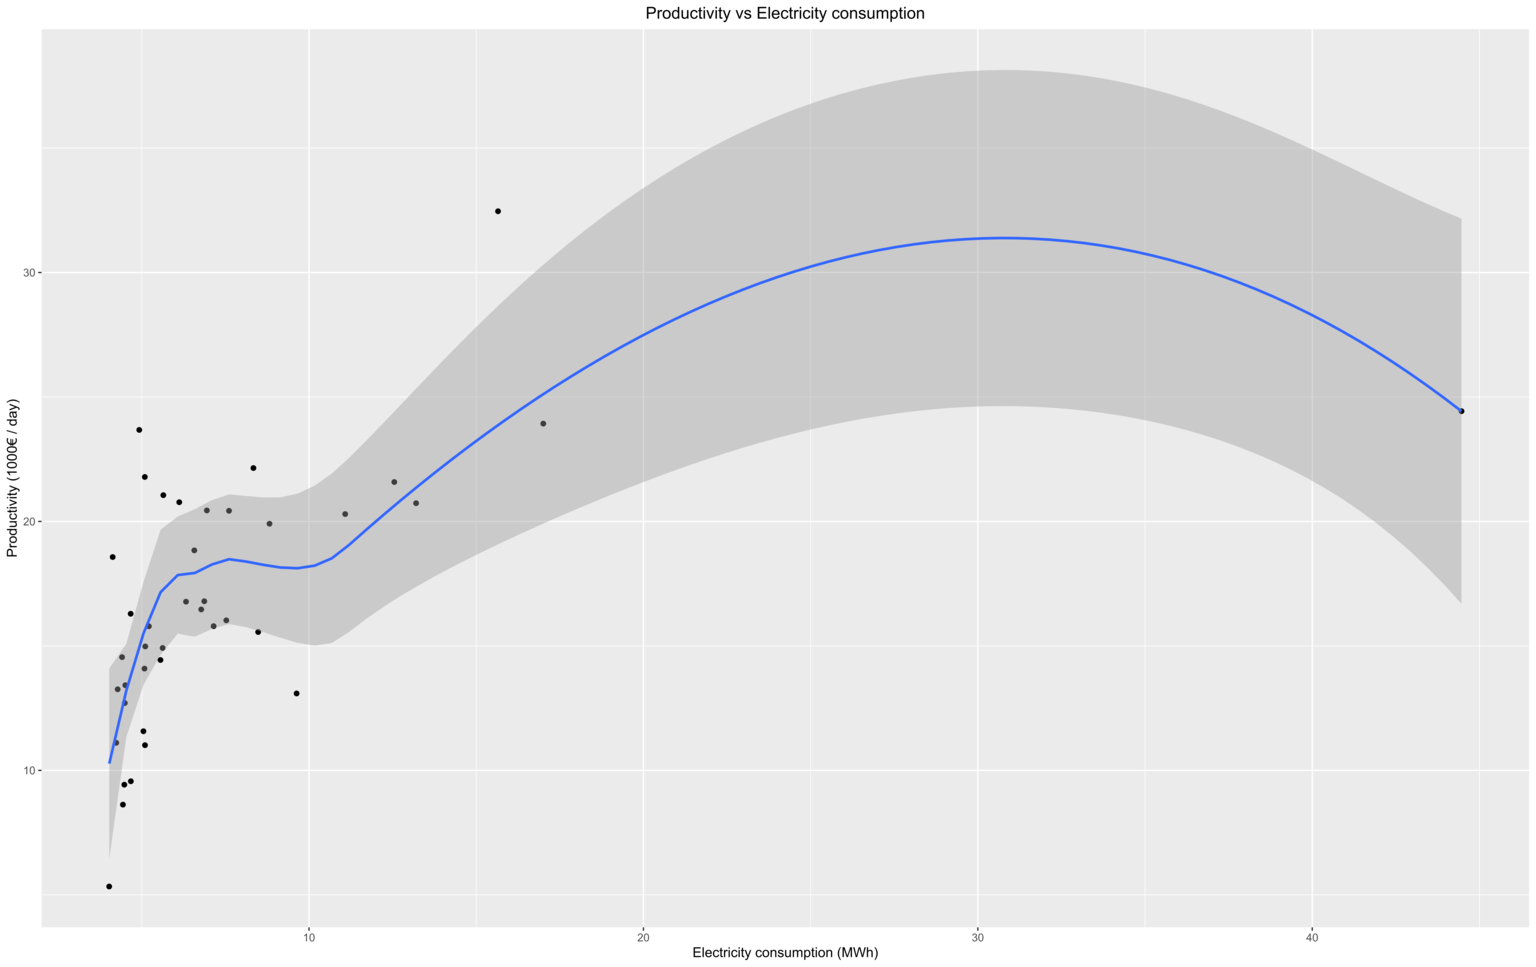
\includegraphics[width=\textwidth]{figures/png/lm_scatter_plot.png}
  \caption{scatter plot of productivity versus electricity consumption}
  \label{fig:scatter_plot}
\end{figure}

\subsection{Linear model: analysis}

\begin{figure}[H]
  \centering
  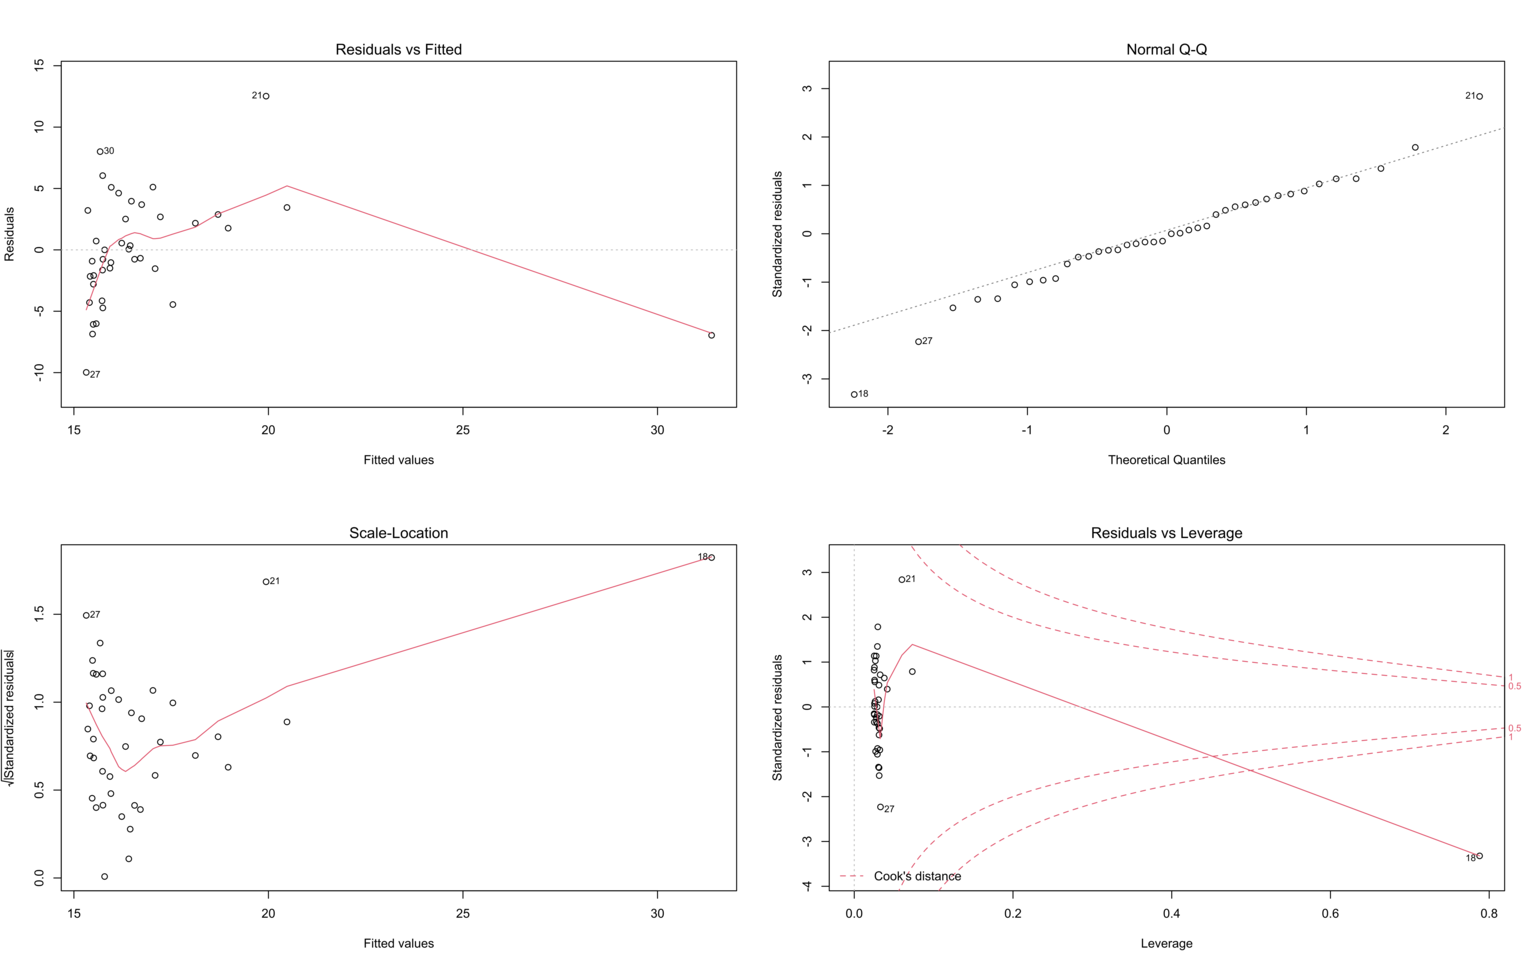
\includegraphics[width=\textwidth]{figures/png/lm_analysis.png}
  \caption{Analysis of the linear model $Y \sim X$}
  \label{fig:analysis-linear-model}
\end{figure}

\subsection{Linear model: histogram of explanatory variable}

\begin{figure}[H]
  \centering
  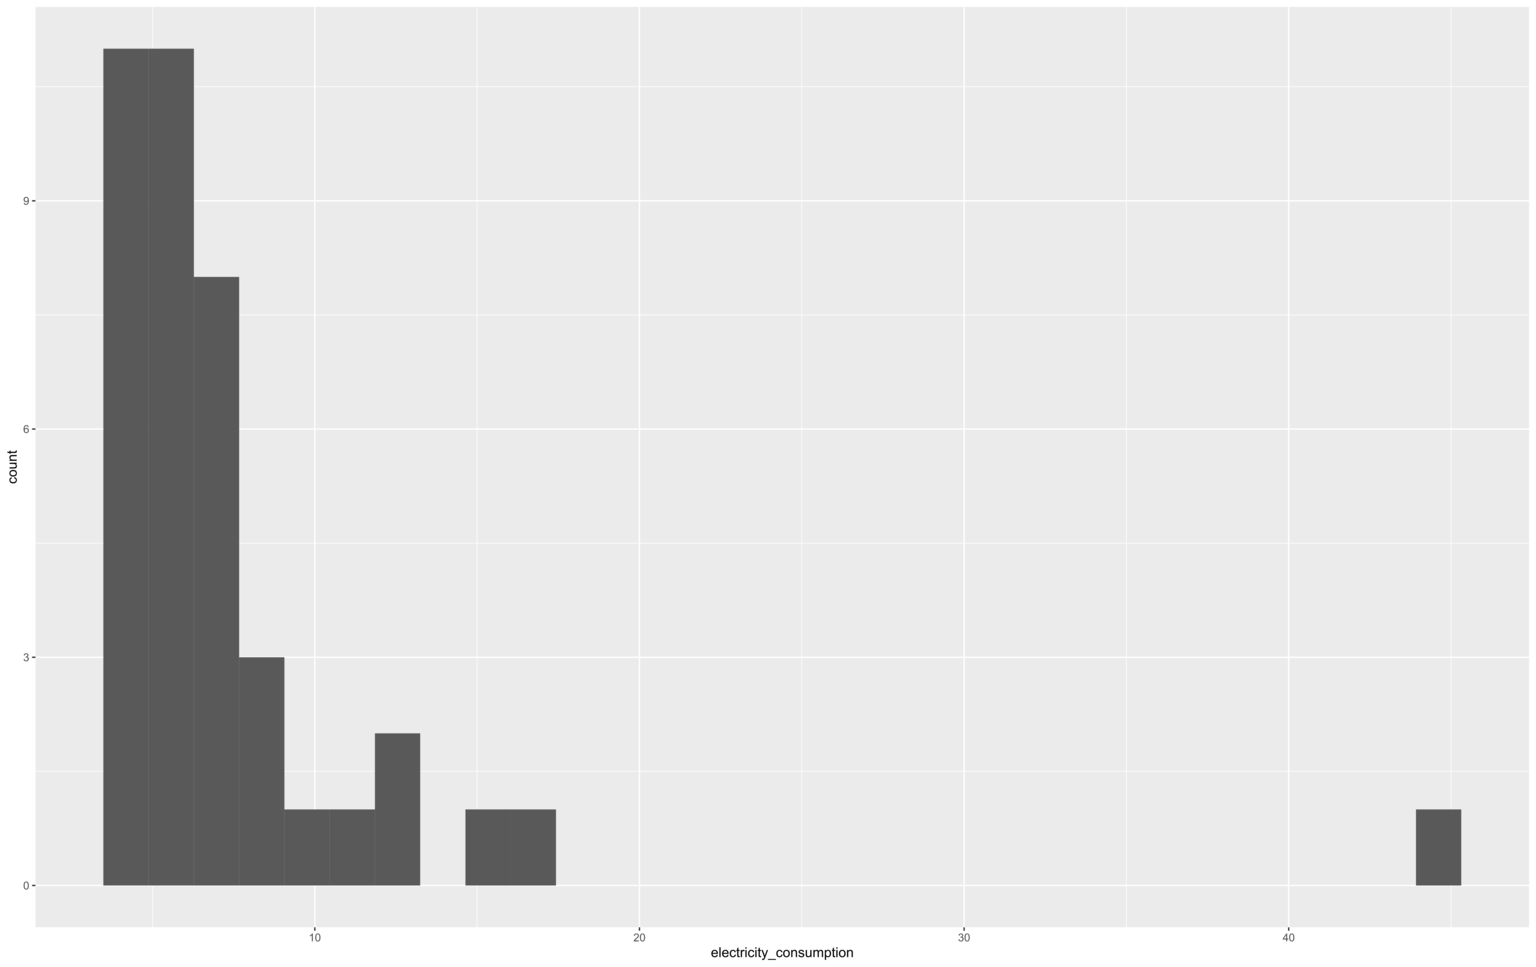
\includegraphics[width=\textwidth]{figures/png/histogram_explanatory_variable.png}
  \caption{Histogram of the explanatory variable $X$ (electricity consumption)}
  \label{fig:histogram-explanatory-variable}
\end{figure}

\subsection{Reciprocal model: scatter plot}

\begin{figure}[H]
  \centering
  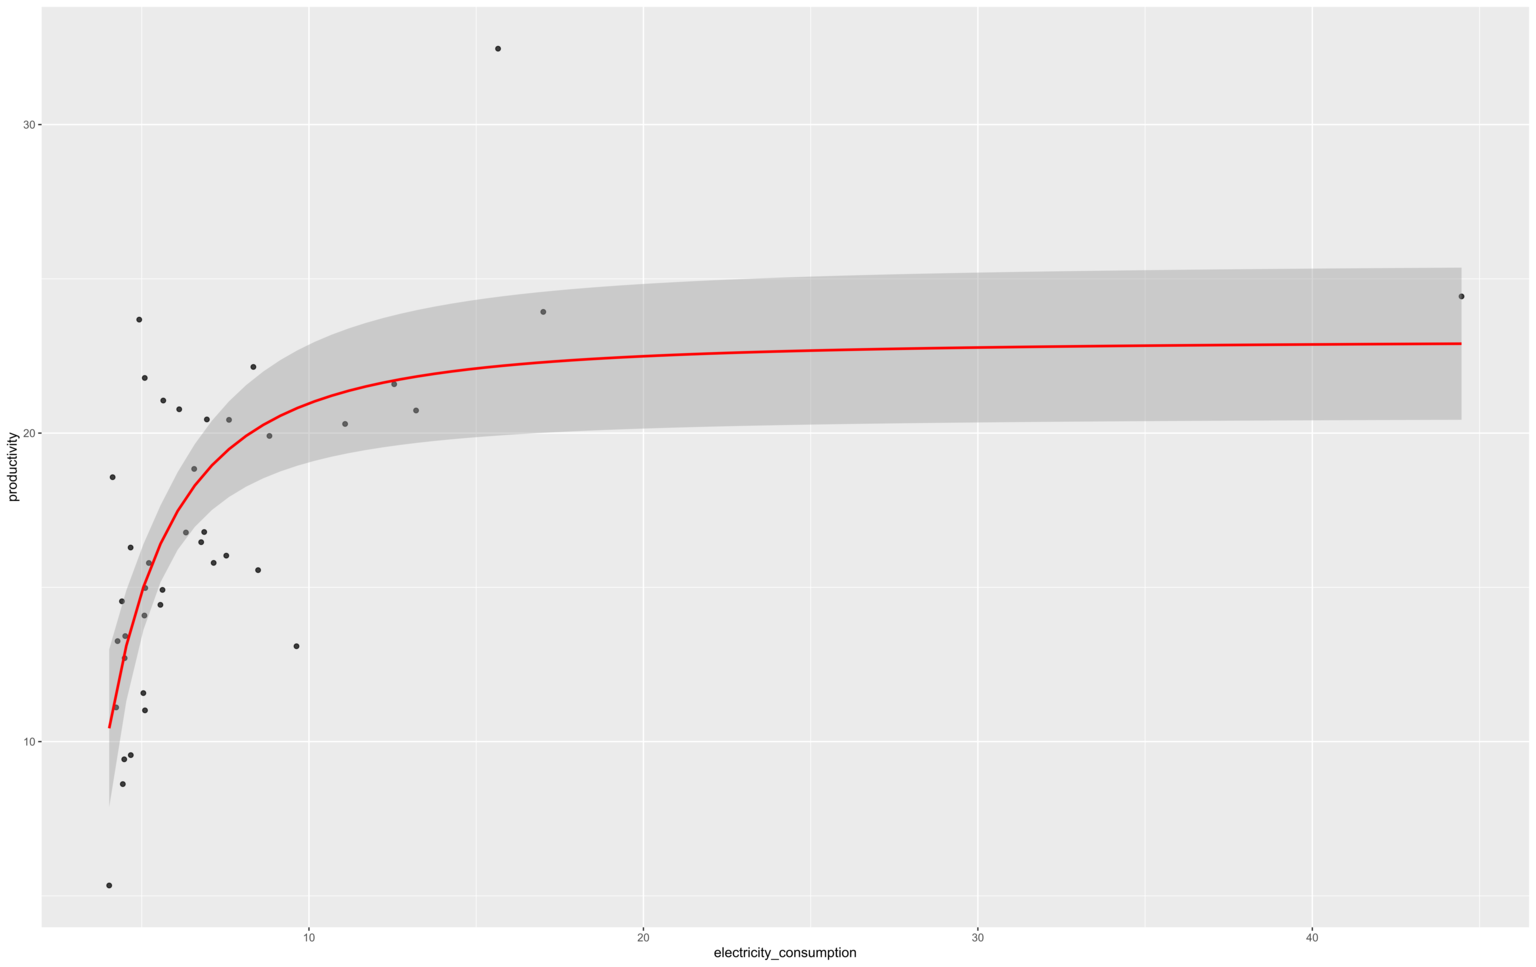
\includegraphics[width=\textwidth]{figures/png/reciprocal_scatter_plot.png}
  \caption{Scatter plot of $Y$ versus $X$. In red we have the following regression line: $Y_i = \beta_0 + \beta_1 (1/(X_i)^2)$}
  \label{fig:scatter-plot-reciprocal-model}
\end{figure}

\subsection{Reciprocal model: linear scatter plot}

\begin{figure}[H]
  \centering
  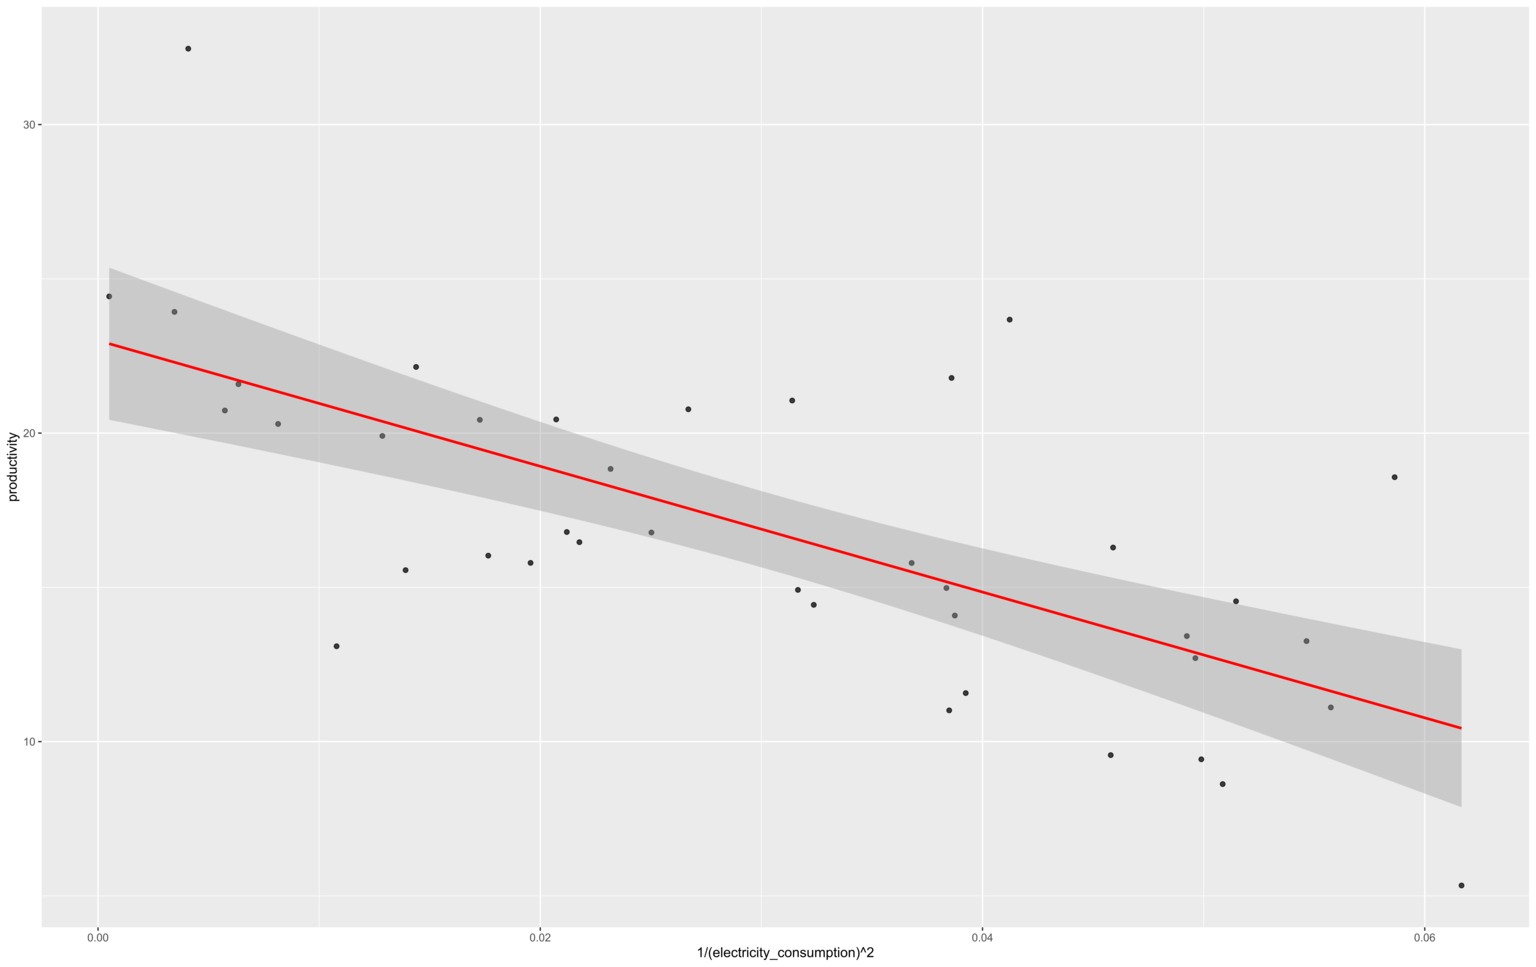
\includegraphics[width=\textwidth]{figures/png/reciprocal_linear_scatter_plot.png}
  \caption{Scatter plot of $Y$ versus $1/X^2$. In red we have the following regression line: $Y_i = \beta_0 + \beta_1 (1/(X_i)^2)$}
  \label{fig:linear-scatter-plot-reciprocal-model}
\end{figure}

\subsection{Reciprocal model: analysis}

\begin{figure}[H]
  \centering
  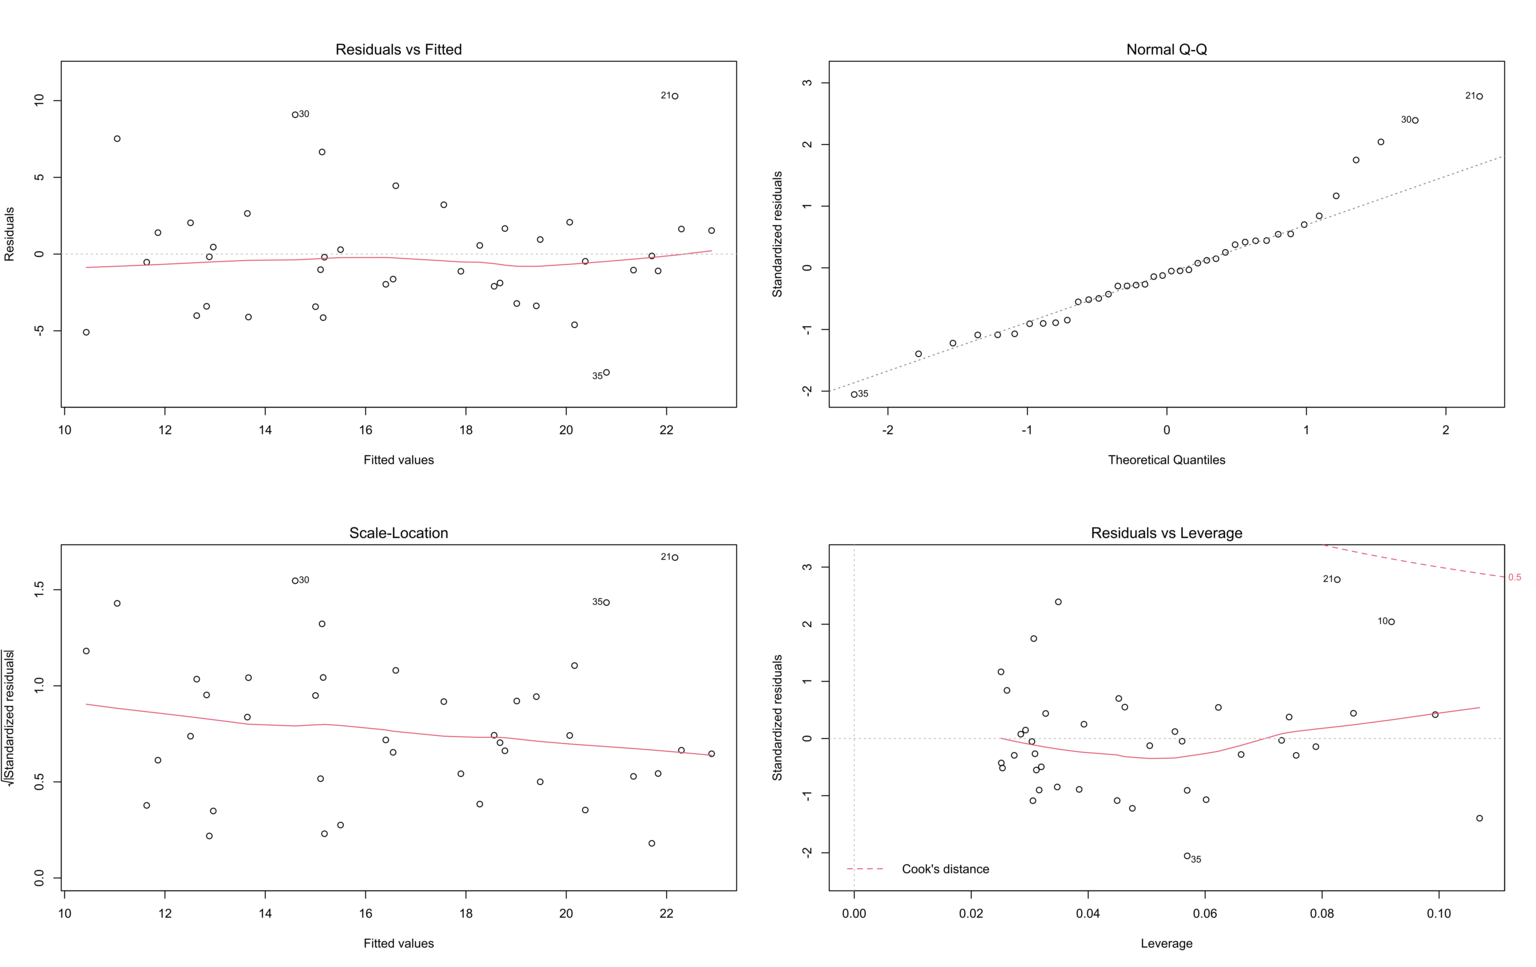
\includegraphics[width=\textwidth]{figures/png/reciprocal_model_analysis.png}
  \caption{Analysis of the model: $Y \sim 1/X^2$}
  \label{fig:reciprocal-model-analysis}
\end{figure}

\subsection{Reciprocal model: summary}

\begin{figure}[H]
  \centering
  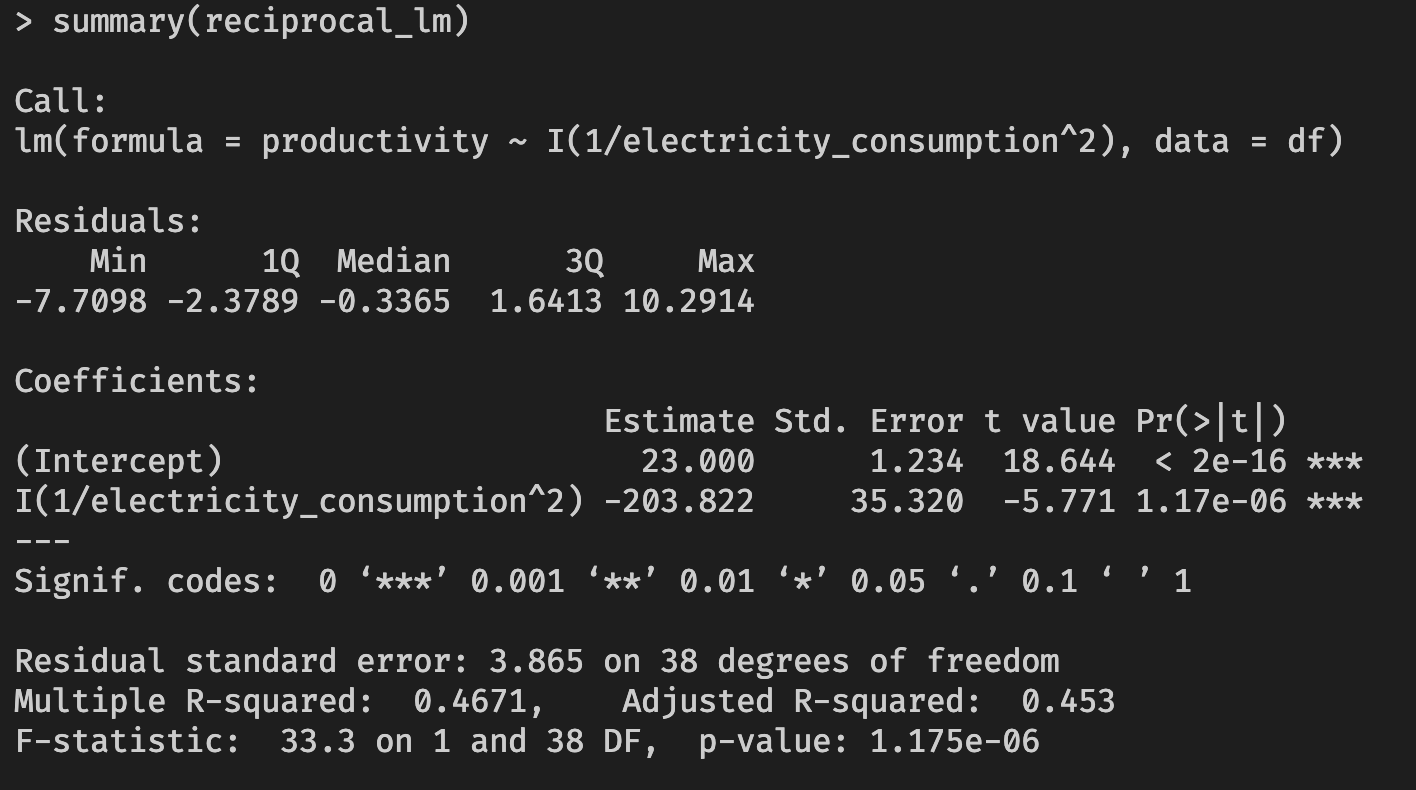
\includegraphics[width=\textwidth]{figures/png/reciprocal-model-summary.png}
  \caption{Summary of the model: $Y \sim 1/X^2$}
  \label{fig:reciprocal-model-summary}
\end{figure}

\section{R code}
\subsection{utils.r}

\begin{minted}{R}
theta_1 <- 3
theta_2 <- 1

# cumulative density function
cdf <- function(x) {
  (-1 / x^3)
}

# inverse of cumulative density function
inv_cdf <- function(y) {
  (1 / ((1 - y)^(1 / 3)))
}

# generate random variables vector from the inverse cdf
inverse_transform_sampling <- function(n, inv_cdf) {
  # generate randoms numbers from the uniform distribution U(0,1)
  data_unif <- runif(n)
  rv_vector <- inv_cdf(y = data_unif)
}

# maximum likelihood method for gini coefficient estimator
gini_mle <- function(rv_vector, n) {
  return(1 / (( (2 * n) / (sum(log(rv_vector / min(rv_vector)))) ) - 1))
}

# method of moment for gini coefficient estimator
gini_mme <- function(rv_vector, n) {
  return(1 / (( (2 * ((n * mean(rv_vector)) - min(rv_vector))) / (n * (mean(rv_vector) - min(rv_vector))) ) - 1))
}

gini_theoretical <- function(theta_1) {
  return(1 / ((2 * theta_1) - 1))
}

bias <- function(sample, theoretical) {
  mean(sample) - theoretical
}

mse <- function(sample, theoretical) {
  mean((sample - theoretical)^2)
}

# x: simulation of sample size n
compute_statistical_quantities <- function(x, n) {
  mean <- mean(x)

  gini_mle_estimator <- gini_mle(rv_vector = x, n = n)
  gini_mme_estimator <- gini_mme(rv_vector = x, n = n)

  c(
    mean,
    gini_mle_estimator,
    gini_mme_estimator
  )
}

# N: simulation size (i.e. number of samples)
# n: sample size
# f: function to generate random variables
# ... any other parameters given to f
sim <- function(N = 1000, n = 20, f, ...) {
  # compute a matrix of random variables based on the distribution f
  # each column correspond to one simulation
  x <- matrix(f(N * n, ...), nrow = n)

  # for each column (i.e. each simulation of sample size n)
  # we compute statistical quantities (mean, gini estimators,...)
  # the function "FUN" is called for each column
  stats <- apply(
    X = x,
    MARGIN = 2,
    FUN = compute_statistical_quantities,
    n = n
  )

  rownames(stats) <- c("mean-sample", "gini-mle-sample", "gini-mme-sample")

  return(stats)
}
\end{minted}

\subsection{code for part. 1}

\begin{minted}{R}
library(tidyverse)
library(reshape2)
library(latex2exp)

setwd("/Users/mathieu/Lab/company-electricity-statistical-analysis/src/")
source("utils.r")

# set a seed for reproductability
set.seed(42)

# Generate sample of size n = 20 by using inverse transform sampling
rv_vector <- inverse_transform_sampling(n = 20, inv_cdf = inv_cdf)

# plot an histogram of the random variable vector
par(mfrow = c(1,1))
hist(rv_vector, breaks = 50, freq = FALSE, xlab = "X", main = "random sample")

# compute Gini coefficients
gini_mle(rv_vector = rv_vector, n = 20)
gini_mme(rv_vector = rv_vector, n = 20)

# Generate N = 1000 times the sample
x <- sim(N = 1000, n = 20, f = inverse_transform_sampling, inv_cdf)

gini_mle_sample <- x["gini-mle-sample", ]
gini_mme_sample <- x["gini-mme-sample", ]

# histogram of gini samples
par(mfrow = c(1, 2))
hist(gini_mle_sample, breaks = 50, main = "", xlab = TeX(r"($\hat{G}_{\textrm{MLE}}$)"), col = "darkorange")
abline(v = gini_theoretical(theta_1), col = "darkgreen", lty = 2)
hist(gini_mme_sample, breaks = 50, main = "", xlab = TeX(r"($\hat{G}_{\textrm{MME}}$)"), col = "steelblue")
abline(v = gini_theoretical(theta_1), col = "darkgreen", lty = 2)
legend("topright", c("Gini MLE", "Gini MME", "True Gini"), fill = c("darkorange", "steelblue", "darkgreen"))

# boxplot of gini samples
par(mfrow = c(1, 2))
boxplot(gini_mle_sample, col = "grey", ylab = TeX(r"($\hat{G}_{\textrm{MLE}}$)"))
abline(h = gini_theoretical(theta_1), col = "darkgreen", lty = 2)
boxplot(gini_mme_sample, col = "grey", ylab = TeX(r"($\hat{G}_{\textrm{MME}}$)"))
abline(h = gini_theoretical(theta_1), col = "darkgreen", lty = 2)

bias_mle <- bias(sample = gini_mle_sample, theoretical = gini_theoretical(theta_1))
bias_mme <- bias(sample = gini_mme_sample, theoretical = gini_theoretical(theta_1))

variance_mle <- var(gini_mle_sample)
variance_mme <- var(gini_mme_sample)

mse_mle <- mse(sample = gini_mle_sample, theoretical = gini_theoretical(theta_1))
mse_mme <- mse(sample = gini_mme_sample, theoretical = gini_theoretical(theta_1))

print(bias_mle)
print(variance_mle)
print(mse_mle)

print(bias_mme)
print(variance_mme)
print(mse_mme)

sample_sizes <- c(20, 40, 60, 80, 100, 150, 200, 300, 400, 500) 

statistical_quantities <- c("gini-bias-mle", "gini-bias-mme", "gini-variance-mle", "gini-variance-mme", "gini-mse-mle", "gini-mse-mme")

matrix <- matrix(NA, nrow = length(statistical_quantities), ncol = length(sample_sizes))
rownames(matrix) <- statistical_quantities
colnames(matrix) <- sample_sizes

# create the different samples, one for each sample size n
for (n in sample_sizes) {
  x <- sim(N = 1000, n = n, f = inverse_transform_sampling, inv_cdf)

  gini_mle_sample <- x["gini-mle-sample", ]
  gini_mme_sample <- x["gini-mme-sample", ]

  bias_mle <- bias(sample = gini_mle_sample, theoretical = gini_theoretical(theta_1))
  bias_mme <- bias(sample = gini_mme_sample, theoretical = gini_theoretical(theta_1))

  variance_mle <- var(gini_mle_sample)
  variance_mme <- var(gini_mme_sample)

  mse_mle <- mse(sample = gini_mle_sample, theoretical = gini_theoretical(theta_1))
  mse_mme <- mse(sample = gini_mme_sample, theoretical = gini_theoretical(theta_1))

  matrix[, as.character(n)] <- c(bias_mle, bias_mme, variance_mle, variance_mme, mse_mle, mse_mme)
}

# create dataframes
bias_df <- data.frame(n = sample_sizes, mle = matrix["gini-bias-mle", ], mme = matrix["gini-bias-mme", ])
var_df <- data.frame(n = sample_sizes, mle = matrix["gini-variance-mle", ], mme = matrix["gini-variance-mme", ])
mse_df <- data.frame(n = sample_sizes, mle = matrix["gini-mse-mle", ], mme = matrix["gini-mse-mme", ])

# converting to long format for easier plotting
bias_df <- melt(bias_df, id = "n")
var_df <- melt(var_df, id = "n")
mse_df <- melt(mse_df, id = "n")

par(mfrow = c(1,1))

# we compare the gini estimators through a plot as a function of n
ggplot(bias_df, aes(x = n, y = value, color = variable)) +
  geom_point() + 
  geom_line() +
  labs(x = "n", y = "bias") +
  scale_fill_hue(labels = c("Gini MLE bias", "Gini MME bias")) +
  theme(legend.title = element_blank())

ggplot(var_df, aes(x = n, y = value, color = variable)) +
  geom_point() + 
  geom_line() +
  labs(x = "n", y = "variance") +
  scale_fill_hue(labels = c("Gini MLE: variance", "Gini MME: variance")) +
  theme(legend.title = element_blank())

ggplot(mse_df, aes(x = n, y = value, color = variable)) +
  geom_point() + 
  geom_line() +
  labs(x = "n", y = "mean squared error") + 
  scale_fill_hue(labels = c("Gini MLE: mse", "Gini MME: mse")) +
  theme(legend.title = element_blank())

sim_n20 <- sim(N = 1000, n = 20, f = inverse_transform_sampling, inv_cdf)
result_n20 <- sqrt(20) * (sim_n20["gini-mle-sample", ] - gini_theoretical(theta_1))

sim_n100 <- sim(N = 1000, n = 100, f = inverse_transform_sampling, inv_cdf)
result_n100 <- sqrt(100) * (sim_n100["gini-mle-sample", ] - gini_theoretical(theta_1))

sim_n500 <- sim(N = 1000, n = 500, f = inverse_transform_sampling, inv_cdf)
result_n500 <- sqrt(500) * (sim_n500["gini-mle-sample", ] - gini_theoretical(theta_1))

par(mfrow = c(1, 3))
hist(result_n20, breaks = 50, main = "sample size: n = 20", xlab = TeX(r"($\sqrt{n}(\hat{G}_{\textrm{MLE}} - G_{\theta_1^0, \theta_2^0})$)"), col = "coral")
hist(result_n100, breaks = 50, main = "sample size: n = 100", xlab = TeX(r"($\sqrt{n}(\hat{G}_{\textrm{MLE}} - G_{\theta_1^0, \theta_2^0})$)"), col = "aquamarine3")
hist(result_n500, breaks = 50, main = "sample size: n = 500", xlab = TeX(r"($\sqrt{n}(\hat{G}_{\textrm{MLE}} - G_{\theta_1^0, \theta_2^0})$)"), col = "steelblue")
\end{minted}

\subsection{code for part. 2}

\begin{minted}{R}
library(tidyverse)

setwd("/Users/mathieu/Lab/company-electricity-statistical-analysis/src/")
df <- read.csv2(file = "electricity_consumption_dataset.txt", sep = ";", dec = ".")
head(df)

df <- rename(df, electricity_consumption = X, productivity = Y)

ggplot(df, aes(x = electricity_consumption, y = productivity)) +
  geom_jitter() +
  geom_smooth() +
  ggtitle("Productivity vs Electricity consumption") +
  xlab("Electricity consumption (MWh)") +
  ylab("Productivity (1000 euros / day)") + 
  theme(plot.title = element_text(hjust = 0.5))

simple_lm <- lm(productivity ~ electricity_consumption, data = df)

par(mfrow = c(2,2))
plot(simple_lm)

summary(simple_lm)

ggplot(df, aes(electricity_consumption)) +
  geom_histogram()

ggplot(df, aes(productivity)) +
  geom_histogram()

# square root transformation
square_root_lm <- lm(productivity ~ sqrt(electricity_consumption), data = df)
summary(square_root_lm)

par(mfrow = c(2,2))
plot(square_root_lm)

ggplot(df, aes(x = electricity_consumption, y = productivity)) +
  geom_point(alpha = 0.7) +
  geom_point(aes(x = electricity_consumption, y = square_root_lm$fitted.values), color = "red", alpha = 0.5) +
  geom_segment(aes(xend = electricity_consumption, yend = square_root_lm$fitted.values), color = "red", alpha = 0.25, linetype = "dashed")

ggplot(df, aes(x = electricity_consumption, y = productivity)) + 
  geom_point(alpha = 0.75) +
  geom_smooth(method = "lm", formula = y ~ sqrt(x), color = "red")

# log transformation
log_lm <- lm(productivity ~ log(electricity_consumption), data = df)
summary(log_lm)

par(mfrow = c(2,2))
plot(log_lm)

ggplot(df, aes(x = electricity_consumption, y = productivity)) +
  geom_point(alpha = 0.7) +
  geom_point(aes(x = electricity_consumption, y = log_lm$fitted.values), color = "red", alpha = 0.5) +
  geom_segment(aes(xend = electricity_consumption, yend = log_lm$fitted.values), color = "red", alpha = 0.25, linetype = "dashed")

ggplot(df, aes(x = electricity_consumption, y = productivity)) + 
  geom_point(alpha = 0.75) +
  geom_smooth(method = "lm", formula = y ~ log(x), color = "red")

ggplot(df, aes(x = log(electricity_consumption), y = productivity)) + 
  geom_point(alpha = 0.75) +
  geom_smooth(method = "lm", color = "red")

ggplot(df, aes(x = log(electricity_consumption))) +
  geom_histogram()

# reciprocal transformation
reciprocal_lm <- lm(productivity ~ I(1 / electricity_consumption^2), data = df)
summary(reciprocal_lm)

par(mfrow = c(2,2))
plot(reciprocal_lm)

ggplot(df, aes(x = electricity_consumption, y = productivity)) +
  geom_point(alpha = 0.7) +
  geom_point(aes(x = electricity_consumption, y = reciprocal_lm$fitted.values), color = "red", alpha = 0.5) +
  geom_segment(aes(xend = electricity_consumption, yend = reciprocal_lm$fitted.values), color = "red", alpha = 0.25, linetype = "dashed")

ggplot(df, aes(x = electricity_consumption, y = productivity)) + 
  geom_point(alpha = 0.75) +
  geom_smooth(method = "lm", formula = y ~ I(1/x^2), color = "red")

ggplot(df, aes(x = 1 / (electricity_consumption)^2, y = productivity)) + 
  geom_point(alpha = 0.75) +
  geom_smooth(method = "lm", color = "red")

ggplot(df, aes(x = 1 / electricity_consumption)) + 
  geom_histogram()
\end{minted}